\documentclass[11pt,a4paper]{article}

\usepackage[utf8]{inputenc}
\usepackage[T1]{fontenc}
\usepackage[french]{babel}
\usepackage{lmodern}
\usepackage[margin=2.2cm]{geometry}
\usepackage{tabularx}
\usepackage{booktabs}
\usepackage{array}
\usepackage{graphicx}
\usepackage{caption}
\usepackage{xcolor}
\usepackage{float}
\usepackage{fancyhdr}
\usepackage[hidelinks]{hyperref}

\newcolumntype{Y}{>{\raggedright\arraybackslash}X}
\setlength{\parindent}{0pt}
\setlength{\parskip}{0.5em}
\renewcommand{\arraystretch}{1.25}
\captionsetup{font=small,labelfont=bf}

\pagestyle{fancy}
\fancyhf{}
\fancyhead[L]{CamTrust Bank -- TP0.1}
\fancyhead[R]{ECNSA}
\fancyfoot[C]{\thepage}

\title{%
	\textbf{Compte rendu de test de sécurité\\
		sur le réseau de CamTrust Bank}\\[0.5em]
}

\author{%
	\begin{tabular}{@{}c@{\hspace{1cm}}c@{}}
		\normalsize NKOUMOU TJADE Grinnel Germain
		&
		\normalsize ETOUNDI Ferdinand Le Grang
		\\[0.1em]
		\multicolumn{2}{c}{%
			\small Dépôt :
			\href{https://github.com/nkoumougrinnel/enix-ecnsa-labs}
			{github.com/nkoumougrinnel/enix-ecnsa-labs}%
		}
	\end{tabular}%
}

\date{24 octobre 2026}

\begin{document}
	
	\maketitle
	\thispagestyle{empty}
	
	% ------------------------------------------------------------------
	\section{Résumé pour la direction}
	
	L’évaluation porte sur un laboratoire reproduisant le réseau fictif de CamTrust Bank.
	Cinq services ont été analysés : web, FTP, Telnet, SNMP et DNS.
	Les captures révèlent des identifiants récupérables sans déchiffrement sur HTTP, FTP et Telnet.
	SNMP v2c expose la communauté \texttt{public} et des informations système ; les échanges DNS sont lisibles.
	Ces observations révèlent des risques de divulgation d’informations et de compromission des accès.
	La priorité est de migrer vers HTTPS, SFTP ou FTPS, SSH v2 et SNMPv3 chiffré,
	puis de désactiver les anciens protocoles après validation.
	
	 %------------------------------------------------------------------
	\section{Périmètre et autorisation}
	
	\begin{table}[H]
		\centering
		\begin{tabularx}{\linewidth}{>{\bfseries}p{3.6cm}Y}
			\toprule
			Élément & Description \\
			\midrule
			
			Environnement &
			Laboratoire pédagogique reproduisant le réseau fictif de
			CamTrust Bank. Les équipements virtuels sont exécutés dans
			EVE-NG, lui-même installé dans une machine virtuelle hébergée
			sur le poste hôte à l'aide de VMware Workstation. \\
			
			Périmètre &
			Siège de Yaoundé : LAN 10.10.10.0/24, SW-SIEGE, R-SIEGE,
			CLIENT-LINUX et PC-SIEGE.
			Agence de Douala : LAN 10.20.10.0/24 et R-DLA, reliée au siège
			par la liaison privée simulée 172.16.12.0/30.
			Internet simulé : R-FAI et SRV-INTERNET (203.0.113.10). \\
			
			Hors périmètre &
			Tout équipement ou réseau extérieur au laboratoire,
			notamment les infrastructures de production.
			Aucun hôte extérieur au laboratoire n'a été scanné. \\
			
			Type de test &
			Observation passive du trafic à partir de captures de paquets
			analysées avec Wireshark, complétée par des connexions de test
			initiées depuis les postes clients du laboratoire. \\
			
			Date &
			24 octobre 2026. \\
			
			Autorisation &
			Travaux réalisés exclusivement dans le cadre du laboratoire
			pédagogique de la formation à la certification ECNSA,
			sous l'encadrement de l'enseignant M. MOUNIR NJI Amine.
			Les opérations sont limitées aux équipements virtuels
			du périmètre décrit ci-dessus. \\
			
			\bottomrule
		\end{tabularx}
		\caption{Périmètre et cadre de réalisation des tests}
	\end{table}
	
	\subsection*{Outils utilisés}
	
	\begin{table}[H]
		\centering
		\small
		\renewcommand{\arraystretch}{1.15}
		\begin{tabularx}{\linewidth}{
				>{\raggedright\arraybackslash\bfseries}p{3.6cm}
				>{\raggedright\arraybackslash}X
			}
			\toprule
			Outil & Utilisation dans le laboratoire \\
			\midrule
			
			EVE-NG &
			Exécution de la topologie virtuelle.
			Ressources allouées à la VM : 6 Go de RAM et 4 vCPU. \\
			
			VMware Workstation &
			Hébergement de la machine virtuelle EVE-NG. \\
			
			Wireshark &
			Capture et analyse des échanges ARP, DHCP, DNS, TCP,
			HTTP, FTP et SNMP. \\
			
			Cisco IOSv / IOSvL2 &
			Émulation du routeur R-SIEGE et du commutateur SW-SIEGE. \\
			
			MikroTik CHR 7.23.8 &
			Émulation du routeur R-DLA de l'agence de Douala. \\
			
			VyOS &
			Émulation du routeur R-FAI représentant le fournisseur
			d'accès Internet. \\
			
			Ubuntu Server 22.04 &
			Système du serveur SRV-INTERNET
			(Apache, vsftpd et dnsmasq) et du poste CLIENT-LINUX. \\
			
			\texttt{curl}, \texttt{dig},
			\texttt{snmpwalk}, \texttt{telnet} &
			Génération des échanges applicatifs à analyser. \\
			
			\texttt{base64} &
			Décodage de la valeur transmise dans l'en-tête
			HTTP \texttt{Authorization: Basic}. \\
			
			VPCS &
			Émulation des postes légers PC-SIEGE et PC-DLA. \\
			
			\bottomrule
		\end{tabularx}
		\caption{Outils et environnements utilisés dans le laboratoire}
		\label{tab:outils}
	\end{table}
	
	% ------------------------------------------------------------------
	\section{Constats}
	
	\begin{table}[H]
		\centering
		\small
		\renewcommand{\arraystretch}{1.2}
		\begin{tabularx}{\linewidth}{
				>{\raggedright\arraybackslash}p{2.6cm}
				>{\raggedright\arraybackslash}X
				>{\raggedright\arraybackslash}p{2.7cm}
				>{\raggedright\arraybackslash}p{1.8cm}
			}
			\toprule
			Service / protocole &
			Observation dans les captures &
			Remédiation proposée &
			Effort indicatif \\
			\midrule
			
			Espace agents web
			\newline HTTP, port 80 &
			La requête \texttt{GET /admin} et l'en-tête
			\texttt{Authorization: Basic} sont visibles.
			Le décodage de sa valeur avec \texttt{base64 -d}
			révèle l'identifiant \texttt{agent} et son mot de passe. &
			HTTPS (TLS) &
			1 jour \\
			
			\midrule
			
			Transfert de fichiers
			\newline FTP &
			Les commandes \texttt{USER} et \texttt{PASS}
			révèlent l'identifiant \texttt{agentftp}
			et son mot de passe. &
			SFTP (SSH) ou FTPS &
			1 à 2 jours \\
			
			\midrule
			
			Administration du routeur
			\newline Telnet &
			Les identifiants de connexion et les commandes
			saisies sont lisibles dans le flux capturé. &
			SSH v2 &
			1 jour \\
			
			\midrule
			
			Supervision
			\newline SNMP v2c &
			La communauté \texttt{public} est visible.
			Les réponses exposent le nom, la description
			et le contact du routeur. &
			SNMPv3 avec authentification et chiffrement &
			1 jour \\
			
			\bottomrule
		\end{tabularx}
		
		\caption{Synthèse des constats et des remédiations proposées}
		\label{tab:constats}
		
	\end{table}
	
	\subsection*{Preuves}
	
	\begin{figure}[H]
		\centering
		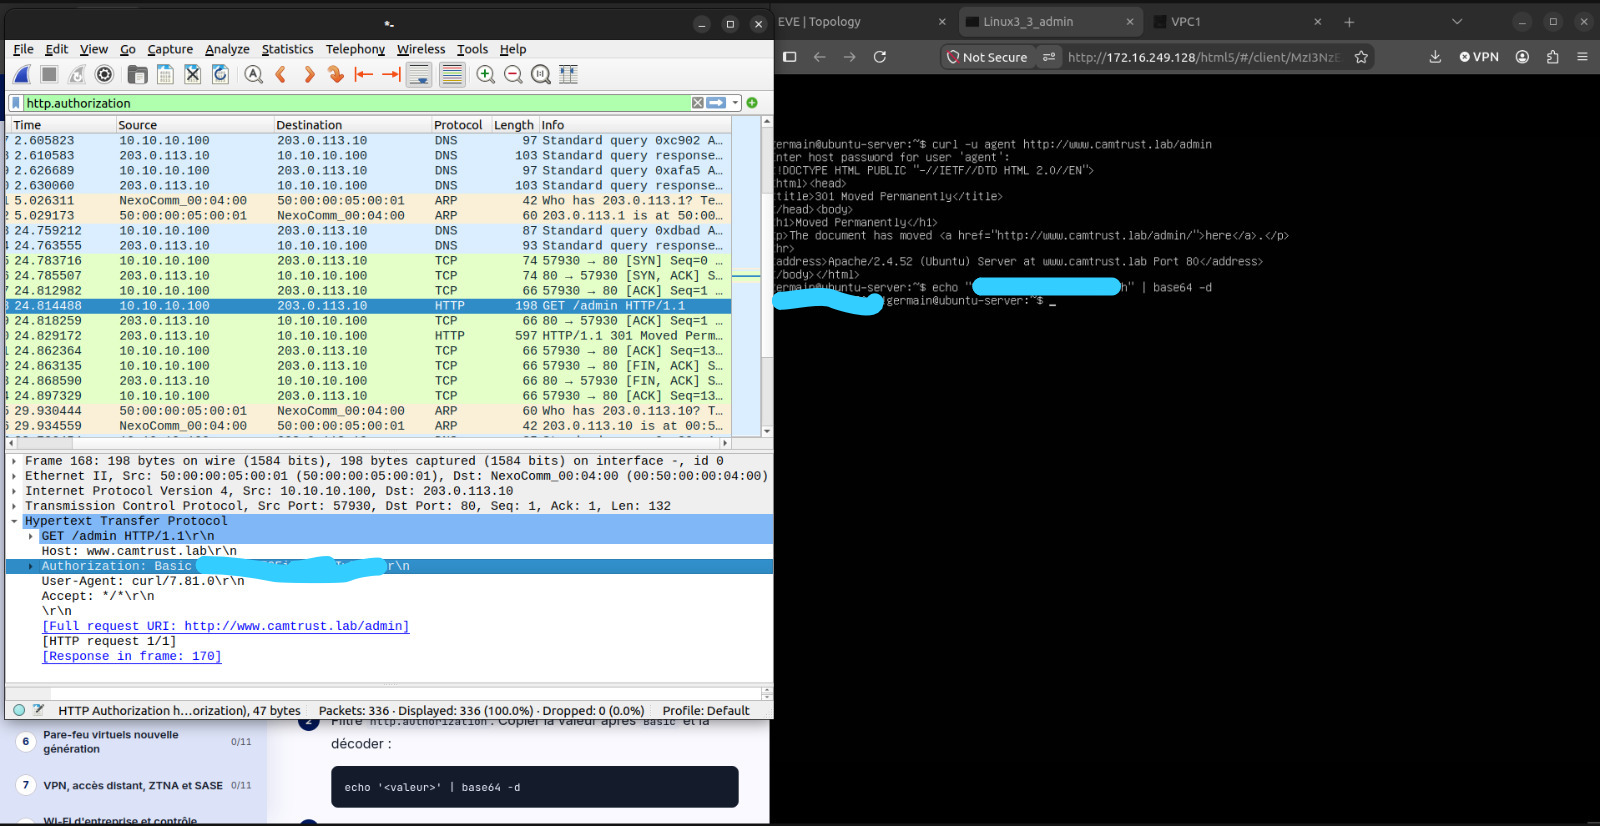
\includegraphics[width=0.8\linewidth]{images/http.png}
		\caption{HTTP : en-tête \texttt{Authorization} visible, identifiant et mot de passe lisibles après décodage (mot de passe flouté).}
	\end{figure}
	
	\begin{figure}[H]
		\centering
		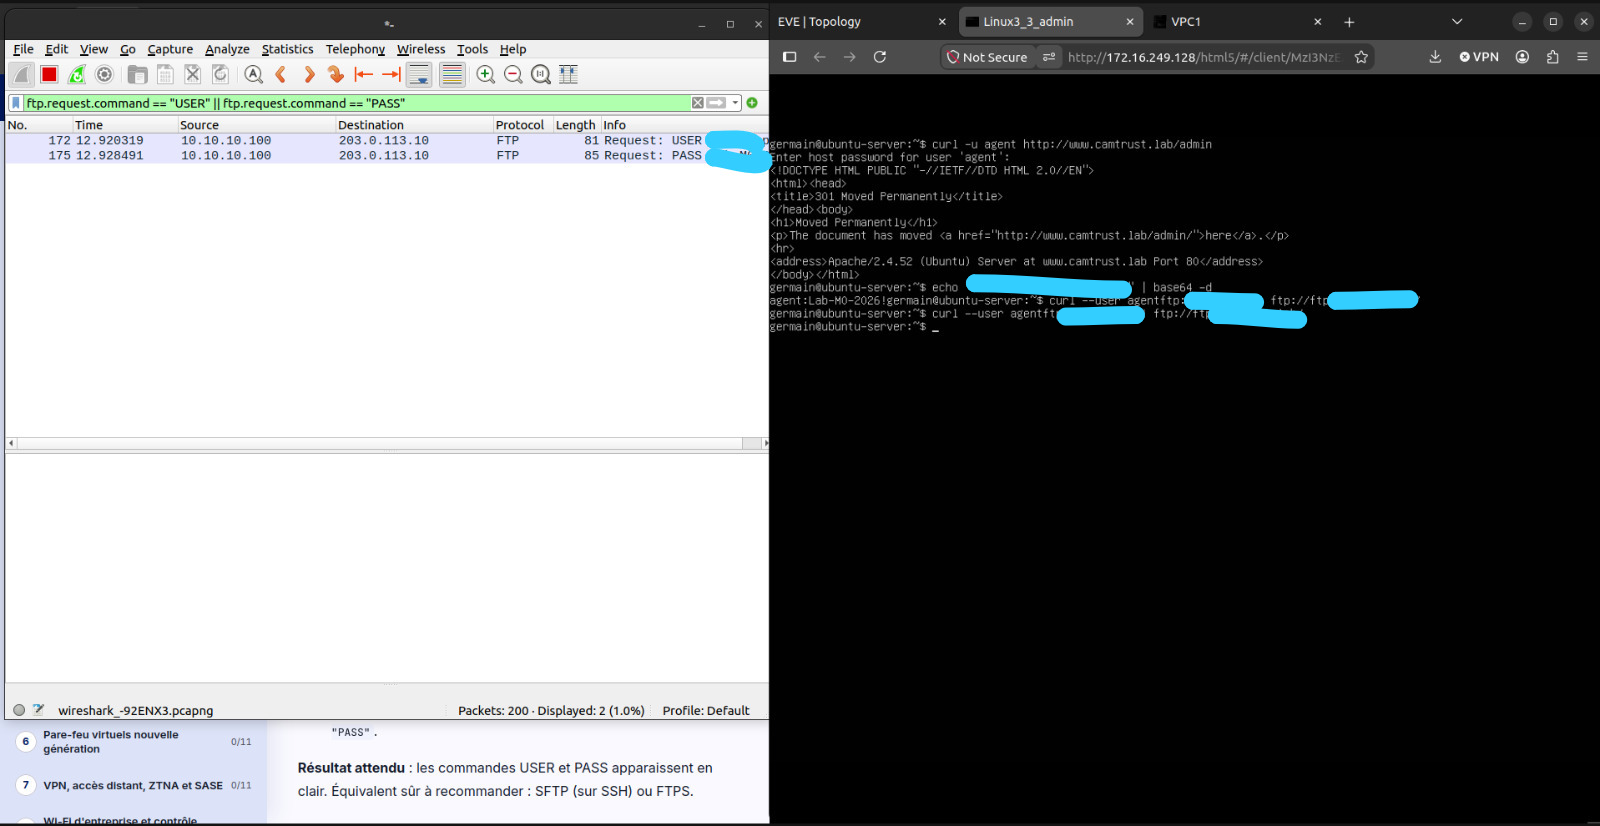
\includegraphics[width=0.8\linewidth]{images/ftp.png}
		\caption{FTP : commandes \texttt{USER} et \texttt{PASS} capturées en clair (identifiants floutés).}
	\end{figure}

	\begin{figure}[H]
		\centering
		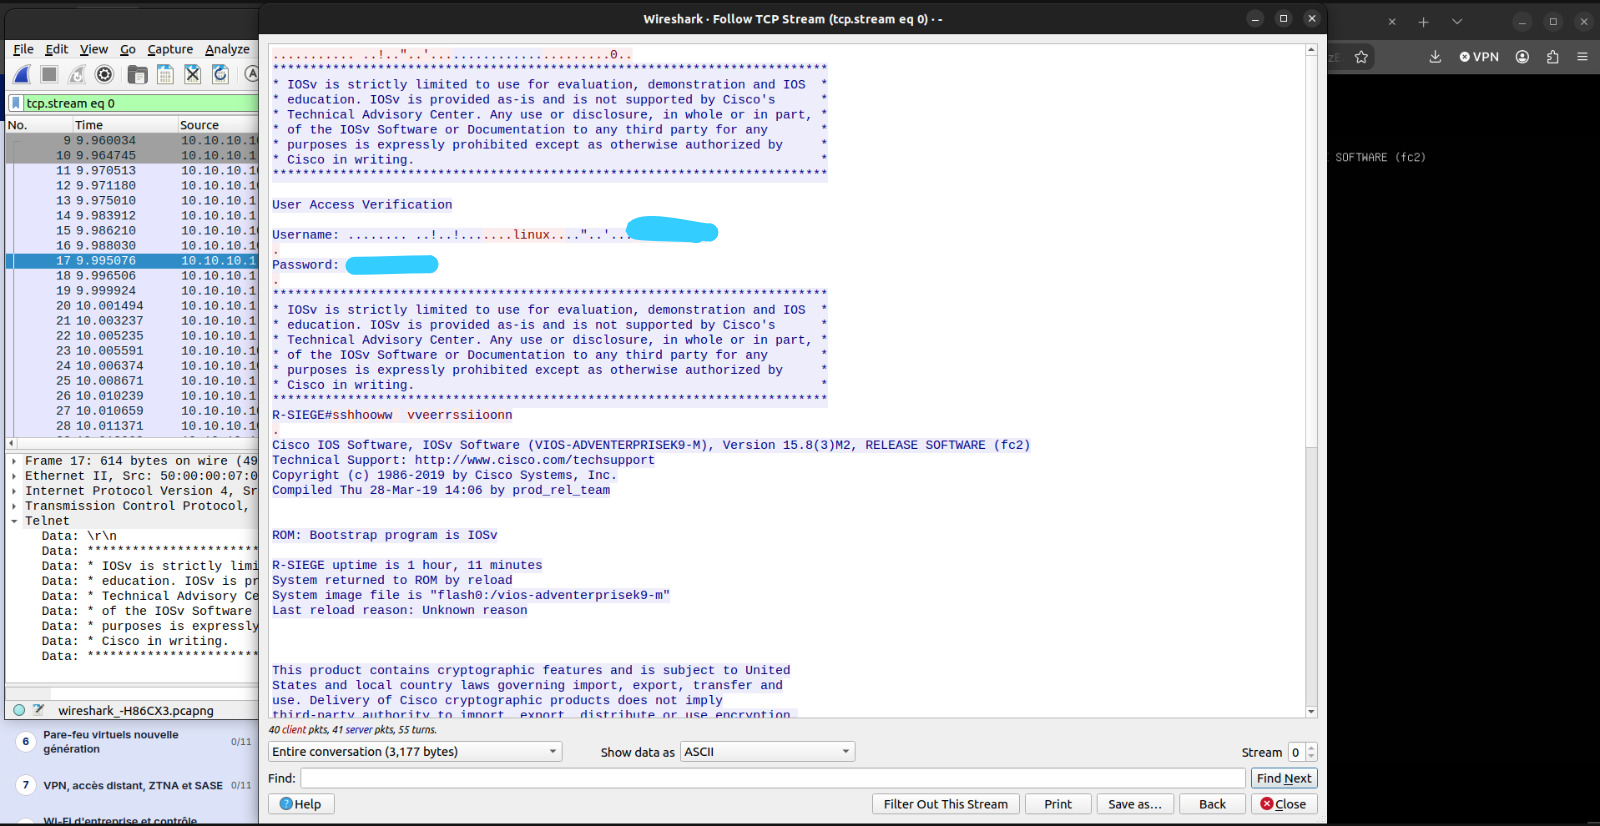
\includegraphics[width=0.8\linewidth]{images/telnet.png}
		\caption{Telnet : identifiants de connexion et commandes d'administration visibles en clair dans la capture.}
	\end{figure}

	
	\begin{figure}[H]
		\centering
		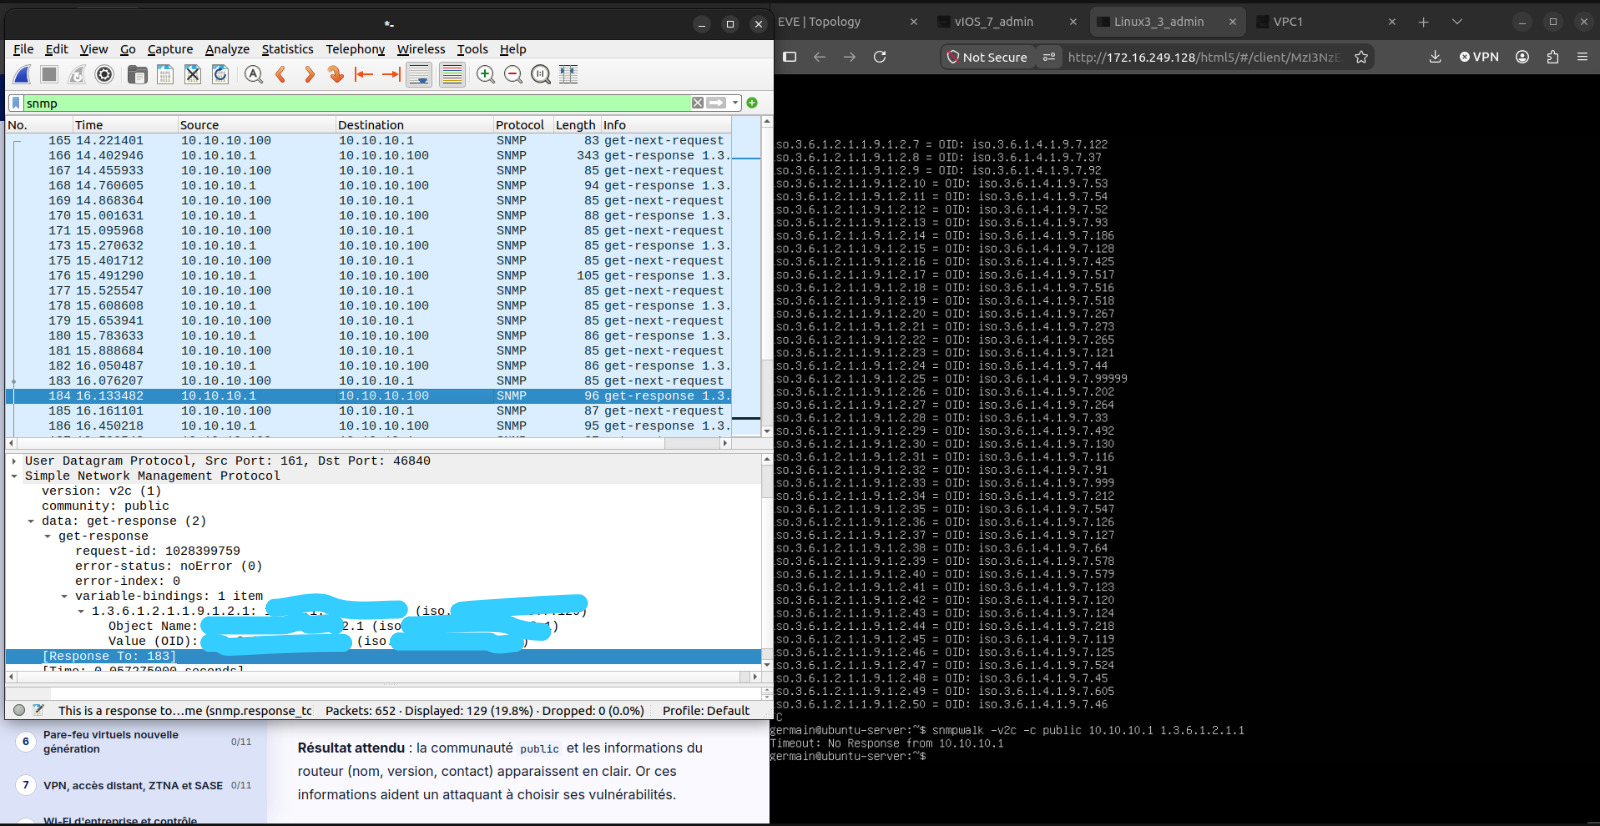
\includegraphics[width=0.8\linewidth]{images/snmp.png}
		\caption{SNMP v2c : communauté \texttt{public} et réponses \texttt{get-response} avec les données système du routeur.}
	\end{figure}
	
	\begin{figure}[H]
		\centering
		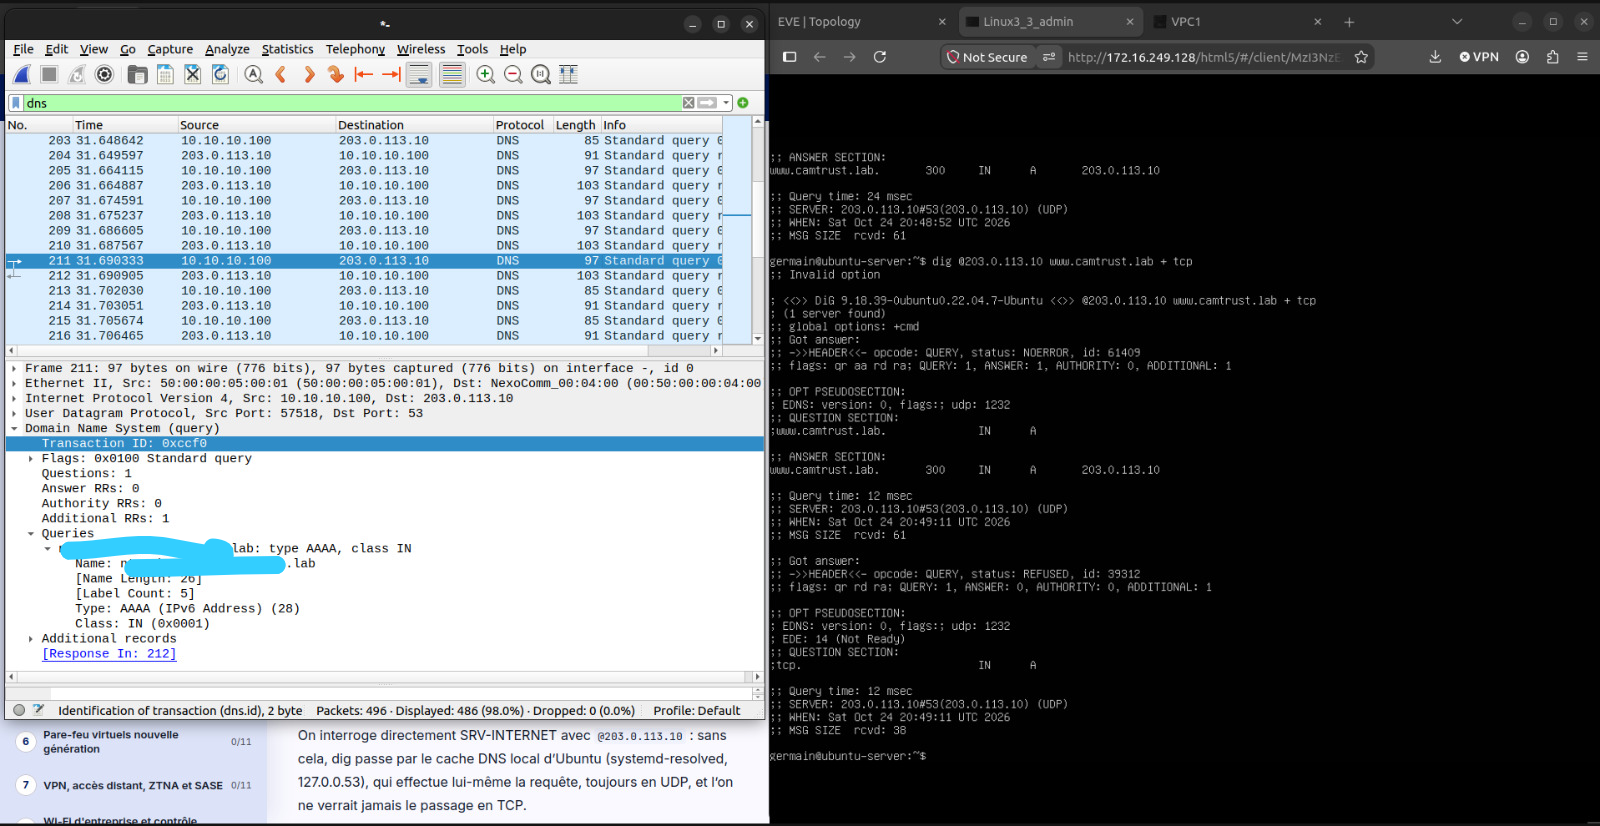
\includegraphics[width=0.8\linewidth]{images/dns.png}
		\caption{DNS : requête et réponse en clair sur UDP 53 (identifiant de transaction visible).}
	\end{figure}
	
	% ------------------------------------------------------------------
	\section{Plan d'action}
	
	\begin{table}[H]
		\centering
		\small
		\renewcommand{\arraystretch}{1.2}
		\begin{tabularx}{\linewidth}{
				>{\raggedright\arraybackslash\bfseries}p{1.3cm}
				>{\raggedright\arraybackslash}X
				>{\raggedright\arraybackslash}X
				>{\raggedright\arraybackslash}p{1.8cm}
				>{\raggedright\arraybackslash}p{1.8cm}
			}
			\toprule
			Service &
			Risque constaté &
			Correction proposée &
			Effort indicatif &
			Module du cours \\
			\midrule
			
			HTTP &
			Identifiants de l'espace agents récupérables
			par un acteur capable d'intercepter le trafic. &
			Déployer HTTPS avec un certificat adapté.
			Après validation, rediriger HTTP vers HTTPS
			et activer HSTS. &
			1 jour &
			 \\
			
			\midrule
			
			FTP &
			Identifiants transmis en clair et absence
			de confidentialité des transferts. &
			Remplacer FTP par SFTP ou FTPS.
			Désactiver le service FTP non chiffré
			après validation des accès et des transferts. &
			1 à 2 jours &
			 \\
			
			\midrule
			
			Telnet &
			Identifiants et commandes d'administration
			visibles dans les échanges capturés. &
			Activer SSH v2 et vérifier les accès.
			Configurer ensuite les lignes VTY avec
			\texttt{transport input ssh} pour interdire Telnet. &
			1 jour,
			hors mise à jour éventuelle &
			 \\
			
			\midrule
			
			SNMP v2c &
			Communauté \texttt{public} et informations
			système visibles dans les captures. &
			Migrer vers SNMPv3 avec authentification
			et chiffrement. Désactiver v2c après validation
			et limiter les accès aux serveurs de supervision. &
			1 jour &
			 \\
			
			\midrule
			
			DNS &
			Noms demandés et réponses DNS visibles
			par un acteur capable d'intercepter les échanges. &
			Étudier le chiffrement des échanges DNS
			avec un résolveur approuvé, notamment
			par DNS-over-TLS, selon les capacités des clients. &
			1 jour
			pour l'étude &
			 \\
			
			\bottomrule
		\end{tabularx}
		
		\caption{Plan d'action proposé à partir des constats du laboratoire}
		\label{tab:plan-action}
		
	\end{table}

	% ------------------------------------------------------------------
	\section{Annexes}

	\begin{itemize}
	\item Configurations finales de R-SIEGE, R-DLA et R-FAI (dossier \texttt{configs/}).
	\item images \texttt{B1-arp.pcapng}, \texttt{B2-dhcp.pcapng}, \texttt{B3-dns.pcapng}, \texttt{B4-tcp.pcapng}.
	\item images \texttt{C1-http.pcapng}, \texttt{C2-ftp.pcapng}, \texttt{C3-telnet.pcapng}, \texttt{C4-snmp.pcapng}.
	\end{itemize}

	\end{document}